%%%%%%%%%%%%%%%%%%%%%%%%%%%%%%%%%%%%%%%%%
% Journal Article
% LaTeX Template
% Version 1.3 (9/9/13)
%
% This template has been downloaded from:
% http://www.LaTeXTemplates.com
%
% Original author:
% Frits Wenneker (http://www.howtotex.com)
%
% License:
% CC BY-NC-SA 3.0 (http://creativecommons.org/licenses/by-nc-sa/3.0/)
%
%%%%%%%%%%%%%%%%%%%%%%%%%%%%%%%%%%%%%%%%%

%----------------------------------------------------------------------------------------
%	PACKAGES AND OTHER DOCUMENT CONFIGURATIONS
%----------------------------------------------------------------------------------------

\documentclass[twoside]{article}

\usepackage{lipsum} % Package to generate dummy text throughout this template

\usepackage{graphicx}
\usepackage[sc]{mathpazo} % Use the Palatino font
\usepackage[T1]{fontenc} % Use 8-bit encoding that has 256 glyphs
\linespread{1.05} % Line spacing - Palatino needs more space between lines
\usepackage{microtype} % Slightly tweak font spacing for aesthetics

\usepackage[hmarginratio=1:1,top=32mm,columnsep=20pt]{geometry} % Document margins
\usepackage{multicol} % Used for the two-column layout of the document
\usepackage[hang, small,labelfont=bf,up,textfont=it,up]{caption} % Custom captions under/above floats in tables or figures
\usepackage{booktabs} % Horizontal rules in tables
\usepackage{float} % Required for tables and figures in the multi-column environment - they need to be placed in specific locations with the [H] (e.g. \begin{table}[H])
\usepackage{hyperref} % For hyperlinks in the PDF

\usepackage{lettrine} % The lettrine is the first enlarged letter at the beginning of the text
\usepackage{paralist} % Used for the compactitem environment which makes bullet points with less space between them

% ABSTRACT

\usepackage{abstract} % Allows abstract customization
%\renewcommand{\abstractnamefont}{\normalfont\bfseries} % Set the "Abstract" text to bold
%\renewcommand{\abstracttextfont}{\normalfont\small\itshape} % Set the abstract itself to small italic text
\renewcommand{\abstractname}{} % Empry abstract title
\renewenvironment{abstract}
 {\normalsize
  \begin{center}
  %\bfseries \abstractname\vspace{-.5em}\vspace{0pt}
  \end{center}
  \list{}{
    \setlength{\leftmargin}{.0cm}%
    \setlength{\rightmargin}{\leftmargin}%
  }%
  \item\relax}
 {\endlist}

% SECTIONS !!
\usepackage{titlesec} % Allows customization of titles
%\renewcommand\thesection{\Roman{section}} % Roman numerals for the sections
%\renewcommand\thesubsection{\Roman{subsection}} % Roman numerals for subsections
\renewcommand\thesection{\arabic{section}} % arabic numerals for the sections
\renewcommand\thesubsection{\arabic{section}.\arabic{subsection}} % arabic numerals for subsections

\titleformat{\section}[block]{\large\scshape}{\thesection.}{1em}{} % Change the look of the section titles
%\titleformat{\section}[block]{\large\scshape\centering}{\thesection.}{1em}{} % Change the look of the section titles
%raggedright
\titleformat{\subsection}[block]{\large}{\thesubsection.}{1em}{} % Change the look of the section titles
\titleformat{\subsubsection}[block]{\large}{\thesubsubsection.}{1em}{} % Change the look of the section titles

%VARIABLES

\newcommand{\myAuthorName}{Aragats Amirkhanyan}
\newcommand{\myUni}{Hasso Plattner Institute}
\newcommand{\myAuthorEmail}{aragats.amirkhanyan@hpi.de}
\newcommand{\myArticleTitle}{Security analysis based on the test environment}

\newcommand{\myNDS}{Network Designer Service}
\newcommand{\myPLT}{Provision Language Translator}
\newcommand{\myPS}{Provision System}
\newcommand{\myNSA}{Network Security Analyzer}


\usepackage{fancyhdr} % Headers and footers
\pagestyle{fancy} % All pages have headers and footers
\fancyhead{} % Blank out the default header
\fancyfoot{} % Blank out the default footer
\fancyhead[C]{\myArticleTitle}
%$\bullet$ November 2012 $\bullet$ Vol. XXI, No. 1 % Custom header text
\fancyfoot[RO,RE]{Fall 2014 Workshop\thepage} % Custom footer text

%Header and footer Lines
\renewcommand{\headrulewidth}{0.4pt}% Default \headrulewidth is 0.4pt
\renewcommand{\footrulewidth}{0.4pt}% Default \footrulewidth is 0pt

%----------------------------------------------------------------------------------------
%	TITLE SECTION
%----------------------------------------------------------------------------------------

\title{\vspace{-15mm}\fontsize{24pt}{10pt}\selectfont\textbf{\myArticleTitle}} % Article title

\author{
\large
\textsc{\myAuthorName}\\
%\thanks{A thank you or further information}\\[2mm] % Your name
\normalsize \myUni \\ % Your institution
\normalsize \href{mailto:\myAuthorEmail}{\myAuthorEmail} % Your email address
\vspace{-10mm}
}
\date{}

%----------------------------------------------------------------------------------------

\begin{document}
\large %Font size

\maketitle % Insert title

\thispagestyle{fancy} % All pages have headers and footers

%----------------------------------------------------------------------------------------
%	ABSTRACT
%----------------------------------------------------------------------------------------

\begin{abstract}

\noindent 
\large %Font size
Research in the field of Information Security is always faced with the problem of lack of data or a suitable environment. This problem is not limited to research in the field of information security, but also for other areas. For research in the field of information security - is a big problem. Researchers have to find solutions for generate data, constructing a suitable environment, etc. A lot of affords to start the research. In the report, we consider examples of how we in the security group of the chair "Internet Technologies and Systems" solve similar problems. We consider the typical ways of solving them and consider a prototype project that we could help to simplify the implementation of research.
%\lipsum[1] % Dummy abstract text

\end{abstract}

%----------------------------------------------------------------------------------------
%	ARTICLE CONTENTS
%----------------------------------------------------------------------------------------

%\begin{multicols}{2} % Two-column layout throughout the main article text

\section{Introduction}

%\lettrine[nindent=0em,lines=3]{L} orem ipsum dolor sit amet, consectetur adipiscing elit.
%\lipsum[2-3] % Dummy text
Many research projects come from the industrial companies. It is seems that if the company is interested in success result of the research, the should provide all needed information, data, their environment. But they do not it. And obviously, the reason has a secure aspect. Most of researchers have to spend a big part of their time for preparing or generate data, deploy research environments and so on. The lack of the data is a big problem academic world. The preparation stage has quite big overhead of the research work, which could be overcome in some cases. It is not a secret that many researchers do the almost same researches which require the same data, the same environment. And every time they have to invent new bicycle. 

In this report we mostly speak about the problems of the security researches. We mention certain problems which we impact during the security research and the way of solving the problems. The report include the overview the prototype application which the main goal is to simplify the preparation stage of the research and make possible to overcome the research overhead. Despite the fact that the report contains information about security research all of that could be used for solving problems in the research project of other areas.      


\section{Deploy test environment}
Many security network and software analysis research start with preparing the test environment. The test environment is deployed in the most cases as the virtual network with configured hosts, routers, networks and all others resources including users account. The test environment could be deployed on the local computer by using the software for virtualization like the VirtualBox, VmWare Workstation and others or could be deployed on the remote server with installed hypervisor software like VMware vSphere Hypervisor (ESXi).          

The common way to create the developing environment is to do it manually. You have to download image of operation system, install it on the Virtual Machine, configure it, install necessary softwares. The developing environment is usually more complex just one virtual machine, so you have to do the same step several. In some cases you can just clone virtual machine, but you still have to do a lot of manual work.       
  
There are some software which can simplify the process of creating the developing/test environment. One of the them is Vagrant. Vagrant allows to create and configure lightweight, reproducible, and portable development environments. The configured environment could be reused. Vagrant project has the relative project which is called VagrantCloud. The project is hosted on the https://vagrantcloud.com. It is some kind of the catalog of prepared environments. The prepared developing environment is called box.  People could share with community their boxes. Everyone could find the appropriate environment and reuse it instead of configuring new one. Vagrant allows to deploy the environment into the local VirtualBox, VMware Workstation, Aamazon Web Service (AWS). It means researchers are quite free in using the platform. The features of the Vagrant are not bound only by running the environment. The application a lot of give capabilities including synchronizing between the host and guest machine, integration with Chef[*], Puppet[*] and other. Learn more on the official website http://www.vagrantup.com/ 

The process of creating the development/test environment can by simplify by cloud providers. Many cloud providers provide capability easy to install and run virtual machine with any operation systems, configure the network and many other features. The most popular is Amazon Web Service (AWS). AWS is Infrastructure-as-a-Service. AWS provides huge amount of service which could solve any problem.  You could combine any infrastructure service to create the certain development environment. I mentioned just AWS, but the market of cloud providers grows extremely so it is possible find any other. As Vagrant AWS also provide capability to save configuration of the development environment, distribute it and reuse.

But we are talking about the researches with security aspects. It means that results and the process of the research in the most cases must secret. In this case it is not possible to use public cloud providers. Here opensource communities come to help us. There si not sense to tell that opensource communities grow extremely. A lot of big IT companies invest into the opensource projects. Many of these opensource projects are widely spread. They are use everywhere. So it does not go past the cloud technologies. There several opensource cloud platform which could be used for creating own IaaS, PaaS and other. Some of them: OpenStack, OpenNebula,  OpenShift Origin and so on. So clouds become private. For us it means that we could create our test/development environments by using flexibility and capability of cloud services. But still there are some problems and overhead of creating the test/development environments. It could be solved by using the PaaS, but PaaS's are usually designed for specific task mostly for running the infrastructure for web applications in Java, PHP, Ruby and so on. No one does provide flexible platform as a service based on all functionality of infrastructure as a service. We would like to call it Platform as a Infrastructure (PaaI). Jeslastic[*] uses this definition for describing its service, but they include other meaning into this definition.     

        


\section{Simulation of users behaviors}
There is task to analyses the behavior of users to predict attacks or abnormal behavior. There are some algorithms for Attack Prediction based on Machine Learning [http://www.csjournals.com/IJCSC/PDF1-2/51..pdf]. The algorithms could be used for research purposes, in this task the big problem is lack of data. The customer do not want and can not provide Active Directory log files which contains information about user activities. We have to start research since writing the script for simulation user behaviors. 

The Scenario in our case is the description of the network infrastructure, information about users, and scenario of their behavior. To analysis user behaviors by predict algorithms we must have normal scenario and abnormal scenario.  
  
\subsection{Environment description}

Description of a network:
\begin{compactitem}
\item 4 computers.
\item Domain controller. 
\item Wiki Server.
\item DB server.
\end{compactitem}
Users: 
\begin{compactitem}
\item Petrov
\item Ivanov 
\item Smirnov
\item Admin
\end{compactitem}
     
\subsection{Normal scenario}
Figure 1. Usually ordinal users login to their computers. They do it several times per day. All users and admin have an access to Wiki, but Ivanov usually do not use it. Admin usually login to Domain Controller. Other users do not do it, because their do not have an access. Ivanov does not login to wiki, but he has an access. Others users do it. Ivanov sometimes login to DB Server. Others users do not do it, but they have an access.
\begin{figure}[ht!]
\centering
%[width=90mm]
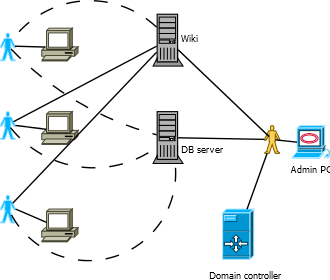
\includegraphics{scenario_normal.png}
\caption{Normal scenario}
\label{overflow}
\end{figure}

\subsection{Abnormal scenario}
Figure 2. Ivanov logged to wiki. He usually does not do it, but he has an access and other users do it every day. Petrov logged to DB server. He has an access, but according to the normal behavior only Ivanov uses the DB server. So it could be abnormal behavior.  

\begin{figure}[ht!]
\centering
%[width=90mm]
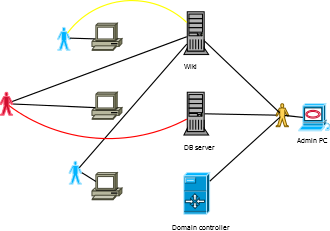
\includegraphics{scenario_abnormal.png}
\caption{Abnormal scenario}
\label{overflow}
\end{figure}

\subsection{Implementation}
The network is deployed and configured manually on the FutureSOC server with WMware ESXi. The script for the simulation users activities is written in Python with using additional libraries for connecting to Virtual Machines by VNC and making screenshots. There are 3 csv files for describing the whole scenario. The first of them (computers.csv) describe the the all computers which participate in the scenario. It contains the information about computer identifier, IP, port, VNC password and type of operation system(OS).
The second (scenarios.csv) describes the main user activity. The main user activity means the connection to the local computer. The files contains computer identifier to connect, username, password, session time, count of sessions and identifier of inner scenario.
The third (inner-scenarios.csv) describes the user activity after login to the local computer. For example, it could describe the connection to the wiki, the DB server or Domain Controller or even connection to another user computer.  
There are two sets of csv files. The first set is used to perform normal scenario and the second is used to perform abnormal scenario 	
accordingly. Normal scenario takes about 3,5 hours and abnormal scenario takes about 5,5 hours.
 

\section{Automatization of research}

\subsection{Motivation}
As we can see from previous sections there is quite big overhead of research in preparing the research environment and performing the basic scenarios. Many researchers usually do common things, scenarios, but for different purpose. Everytime they have to invent new bicycle and in most cases it is just a waste of time. It would be nice to have some tool for overcoming this overhead, to automatize the common research processes and make research easier. We suggest the concept of the project consists of four independent projects. Each project could be used independent and will be useful for researches, users, administrators, developers. Project could be used together or in any combination to solve different research problems. We call the project Security Lab Generator (SLG). It contains four projects (systems): 
\begin{compactitem}
\item \myNDS{ } (ND)
\item \myPLT{ } (PLT)
\item \myPS{ } (PS)
\item \myNSA{ } (NSA)
\end{compactitem}

\begin{figure}[ht!]
\centering
%[width=90mm]
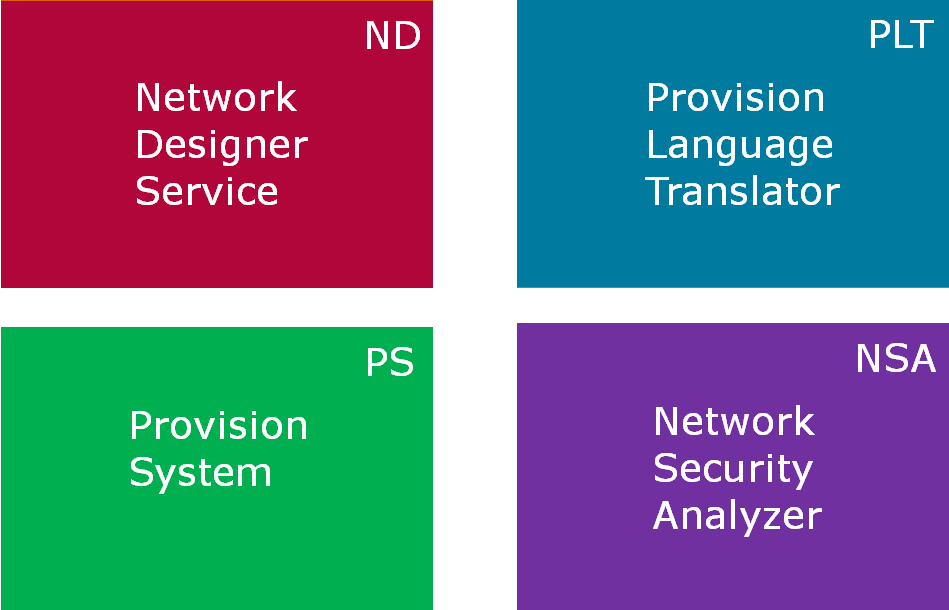
\includegraphics[width=120mm]{slg_structure.png}
\caption{SLG's systems}
\label{overflow}
\end{figure}
 
 
\subsection{\myNDS}
The purpose of the \myNDS{ }is to provide easy way to design the network including specifying networks, hosts, connections, softwares, user accounts. The system should provide the flexibility providing by IaaS and simplicity providing by PaaS. It the first part of the big ecosystem. The system should provide the capability to export designed network as structured data. For example XML, JSON or other. It could be used independently by system administrator to design the network and collaboration. And also it could be used in combination with others system to perform the whole life cycle flow. As we mentioned in the previous subsection we want to create project for automatization of research. So it is the first step to reach goal. 

Research areas:



\subsection{\myPLT}
Some system provide the capability to describe the environment and deploy it. But each system has its own language. If you do not think about using different provision providers then there is not problem. But it could be that you will need think about the migration from one provider to other. For example from Amazon Web Service (AWS) to your own server with VMware EXSi. In this case you have to spend a lot of time to running the same environment on your own servers. To automatize the process you would like some tools like Vagrant, but it can not resolve all problems of migration, because you still have to write instruction for Vagrant manually. To overcome the problem of migration and provide flexibility in choosing the provider for deploying the environment, PLT is suggested. 

PLT is a translator like Google Translator, but not for nature languages, but for provision languages. Provision language is a full description of the environment that cloud be used for deploying described environment according to description. Idea PLT is provide so many module as possible for bi-direction translation provision language. The project could be used independently by system administrators for migration network environments from on to other provision provider. But in our case we want to use it in combination with other systems. So we should provide the translation from our network description language to already existing language like Vagrant file or Amazon Cloud Formation or other. So now we have 2 systems ND and PLT. We could design the network, export SLG XML and then translate it into appropriate provision language. 

     
Research areas:     

\subsection{\myPS}
Provision system is used for deploying the environment based on the description. It can accept different different types of provision language and provide provision on different providers: AWS? OpenStack, VmWare, VirtualBox and so on. It PS can directly apply provision language to provider of you PLT service to translate input provision language to appropriate for certain provider and then apply it. In combination of three described system we could design the network, convert to appropriate provision language and apply to certain provider. 

Research areas:


\subsection{\myNSA}
Network system analyzer is the most interesting part of the project, because it is used for making research, gathering data from host, scanning the host, analyze data, making report and applying user scenarios. The system contains two parts: server side and agents. The server side is wrapper of many security analytic tools such as MulVal. All tools need data to analyze them and create reports, attack graph and show some statistics. So server must  know about the whole network structure also gather data from the hosts. The first issue could be solved by passing the SLG XML describing designed network from ND. Already on this step NSA can provide information such attack graph and potential vulnerabilities. But is is not enough. We need information about hosts. For this issue we can use agent. The agent could include different inventory, monitoring, suffering tools to make fully analyzing of the host. Some of possible tools: OVAL SCANNER !!!!. The agent registers in the server and ready to send data to server. The server receive data and depending on the time delegate them to the appropriate analytic tool. The system could get access to other services that could provide useful information for making reports and analyzing data. For example the system could work with Vulnerability Database (VDB). 

Other very important purpose is create user scenarios, send them to agent and agent apply them. The system should provide the co     


Research areas:


%------------------------------------------------

\section{Methods}

Maecenas sed ultricies felis. Sed imperdiet dictum arcu a egestas. 
\begin{compactitem}
\item Donec dolor arcu, rutrum id molestie in, viverra sed diam
\item Curabitur feugiat
\item turpis sed auctor facilisis
\item arcu eros accumsan lorem, at posuere mi diam sit amet tortor
\item Fusce fermentum, mi sit amet euismod rutrum
\item sem lorem molestie diam, iaculis aliquet sapien tortor non nisi
\item Pellentesque bibendum pretium aliquet
\end{compactitem}
\lipsum[4] % Dummy text

%------------------------------------------------

\section{Results}

\begin{table}[H]
\caption{Example table}
\centering
\begin{tabular}{llr}
\toprule
\multicolumn{2}{c}{Name} \\
\cmidrule(r){1-2}
First name & Last Name & Grade \\
\midrule
John & Doe & $7.5$ \\
Richard & Miles & $2$ \\
\bottomrule
\end{tabular}
\end{table}

\lipsum[5] % Dummy text

\begin{equation}
\label{eq:emc}
e = mc^2
\end{equation}

\lipsum[6] % Dummy text

%------------------------------------------------

\section{Discussion}

\subsection{Subsection One}

\lipsum[7] % Dummy text

\subsection{Subsection Two}

\lipsum[8] % Dummy text

%----------------------------------------------------------------------------------------
%	REFERENCE LIST
%----------------------------------------------------------------------------------------

%\begin{thebibliography}{99} % Bibliography - this is intentionally simple in this template
%
%\bibitem[1]{Figueredo:2009dg}
%Figueredo, A.~J. and Wolf, P. S.~A. (2009).
%\newblock Assortative pairing and life history strategy - a cross-cultural
%  study.
%\newblock {\em Human Nature}, 20:317--330.
% 
%\end{thebibliography}

\input{mylib.bbl}
\bibliographystyle{IEEEtran}
%\bibliographystyle{ieeetr}
\bibliography{mylib}


%----------------------------------------------------------------------------------------

% Multicolumn END
%\end{multicols}

%\bibliography{mylib}

\end{document}
